% Drawing 74/04-2 -- folder 74, batch 04, archive page 61 (PDF page 62).
% Transcription: deux triangles ayant le sommet $a$ en commun.
% Kind: two triangles with a common vertex. Method 3 (encoded, rendered from the data). Status: ok.
% Notes: Two triangles sharing the vertex a. Encoded as polyhedron/1 (two 2-cells glued at a point).
% Coordinates: 1 unit = 1 mm = 1/100 of the crop width (bbox in page fractions: [0.15, 0.68, 0.4, 0.86]).
% Redrawn by Claude (claude-opus-5-5), issue #73, 2026-11-07; not checked by a human; not compiled (no TeX in the session).
% Rights: reproduces part of the work -- behind RENDER_TRANSCRIPTS, never published by itself.
\documentclass[tikz,border=3pt]{standalone}
\usepackage{amsmath,amssymb}
\usetikzlibrary{patterns,arrows.meta}
\tikzset{pencil/.style={black!45}, struck/.style={black!35}, mark/.style={circle,draw,inner sep=1.3pt}, pt/.style={circle,fill,inner sep=0.9pt}, opt/.style={circle,draw,fill=white,inner sep=1.1pt}}
\begin{document}
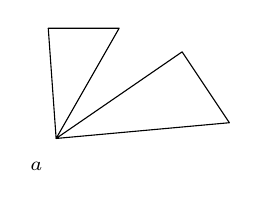
\begin{tikzpicture}[x=1mm,y=1mm,line cap=round,line join=round,font=\scriptsize]
\draw (51,-26) -- (50,-12) -- (59,-12) -- cycle;
\draw (51,-26) -- (67,-15) -- (73,-24) -- cycle;
\node[inner sep=1pt] at (48.5,-29.5) {\scriptsize $a$};
\end{tikzpicture}
\end{document}
